\documentclass[14pt,a4paper]{scrartcl}
\usepackage{cmap}
\usepackage[utf8]{inputenc}
\usepackage[T1,T2A]{fontenc}
\usepackage[english,russian]{babel}
\usepackage{relsize}
\usepackage{graphicx}
\usepackage{subfigure}
\usepackage{mathtools}
\usepackage{amssymb}
\usepackage{float}
\usepackage{sidecap}
\usepackage{wrapfig}
\usepackage{caption}
\usepackage[table,xcdraw]{xcolor}
\usepackage{listings}
\usepackage{amsmath,cryptocode}
\usepackage{listings}
\usepackage{booktabs}
\usepackage{multirow}  
\usepackage{multicol}
\usepackage{bigstrut}
\usepackage{lscape}
\usepackage{rotating}
\usepackage{adjustbox}
\usepackage{minted}


\newcommand\scalemath[2]{\scalebox{#1}{\mbox{\ensuremath{\displaystyle #2}}}}


\begin{document}
	\begin{titlepage}
	\begin{center}
		\large
		МИНИСТЕРСТВО ОБРАЗОВАНИЯ И НАУКИ\\ РОССИЙСКОЙ ФЕДЕРАЦИИ
		
		\vspace{0.5cm}
		
		МГТУ им Н.Э.Баумана
		\vspace{0.25cm}
		
		Факультет ФН
		
		Кафедра вычислительной математики и математической физики
		\vfill
		
		
		Соколов Арсений Андреевич\\
		\vfill
		
		
		{\LARGE Лабораторная работа №3 по численным методам\\[2mm]
		}
		\bigskip
		
		3 курс, группа ФН11-53Б\\
		Вариант 6
	\end{center}
	\vfill
	
	\newlength{\ML}
	\settowidth{\ML}{«\underline{\hspace{0.7cm}}» \underline{\hspace{2cm}}}
	\hfill\begin{minipage}{0.4\textwidth}
		Преподаватель\\
		\underline{\hspace{3cm}} В.\,А.~Кутыркин\\
		«\underline{\hspace{0.7cm}}» \underline{\hspace{1.71cm}} 2019 г.
	\end{minipage}%
	\bigskip
	
	
	\vfill
	
	\begin{center}
		Москва, 2019 г.
	\end{center}
\end{titlepage}

\section*{Задание 1.1}
\textbf{Задание.}\\
Используя метод простой итерации с нулевым начальным вектором, найти приближённое решение СЛАУ: $A \cdot \prescript{>}{}{x} = \prescript{>}{}{b}$, с матрицей, имеющей диагональное преобладание. Абсолютная погрешность
приближённого решения не должна превышать величины 0,01. Предполагается, что все компоненты решения заданной СЛАУ равны единице. Матрица $A$ этой СЛАУ приведена ниже в зависимости от варианта задания (см. Таблицы 1а,б). Кроме того, найти в методе простой итерации число шагов, необходимое для того чтобы гарантировать абсолютную погрешность приближённого решения не более 0.01. Сравнить это расчётное количество шагов с реальным количеством шагов, обеспечившим заданную погрешность.\\
\textbf{Исходные данные.}\\
$N = 6, n = 53$

$$ A =
\begin{pmatrix}
	10\beta & 1  & 2  & 3  \\
	1  & 10\beta & 3  & -2 \\
	2  & 3  & 10\beta & 1  \\
	3  & 2  & 1  & 10\beta
\end{pmatrix}
$$
$$
\prescript{>}{}{x} = 
\begin{pmatrix}
	1 \\
	1 \\
	1 \\
	1
\end{pmatrix}
$$


\textbf{Решение.}\\
Используя рабочую формулу метода простой итерации для решения СЛАУ:
\begin{equation*}
	\prescript{>}{}{x} = F \cdot \prescript{>}{}{x_{(k)}} + \prescript{>}{}{g},
\end{equation*}
где $F = E - D\cdot A$, $\prescript{>}{}{g} = D \cdot \prescript{>}{}{b}$, $k \in \mathbb{N}$.


$$ A =
\begin{pmatrix}
12 & 1  & 2  & 3  \\
1  & 12 & 3  & -2 \\
2  & 3  & 12 & 1  \\
3  & 2  & 1  & 12
\end{pmatrix}
$$

$$ D =
\begin{pmatrix}
0,083333 & 0        & 0        & 0        \\
0        & 0,083333 & 0        & 0        \\
0        & 0        & 0,083333 & 0        \\
0        & 0        & 0        & 0,083333
\end{pmatrix}
$$

$$
\prescript{>}{}{b} = 
\begin{pmatrix}
18 \\
14 \\
18 \\
18
\end{pmatrix}
$$

$$ F =
\begin{pmatrix}
0,000000  & -0,083333 & -0,166667 & -0,250000 \\
-0,083333 & 0,000000  & -0,250000 & 0,166667  \\
-0,166667 & -0,250000 & 0,000000  & -0,083333 \\
-0,250000 & -0,166667 & -0,083333 & 0,000000 
\end{pmatrix}
$$

$$
\prescript{>}{}{g} = 
\begin{pmatrix}
1,5000 \\
1,1667 \\
1,5000 \\
1,5000
\end{pmatrix}
$$

Начальный вектор итераций:

$$
\prescript{>}{}{x_0} = 
\begin{pmatrix}
0 \\
0 \\
0 \\
0
\end{pmatrix}
$$

Получающаяся последовательность приближенных решений СЛАУ:
\begin{equation*}
\prescript{>}{}{x_1} = 
\begin{pmatrix}
1,50000 \\
1,16667 \\
1,50000 \\
1,50000
\end{pmatrix}
\quad
\Delta\prescript{>}{}{x_1} = 0,50000
\end{equation*}

\begin{equation*}
\prescript{>}{}{x_2} = 
\begin{pmatrix}
0,77778 \\
0,91667 \\
0,83333 \\
0,80556
\end{pmatrix}
\quad
\Delta\prescript{>}{}{x_2} = 0,22222
\end{equation*}

\begin{equation*}
\prescript{>}{}{x_3} = 
\begin{pmatrix}
1,08333 \\
1,02778 \\
1,07407 \\
1,08333
\end{pmatrix}
\quad
\Delta\prescript{>}{}{x_3} = 0,08333
\end{equation*}

\begin{equation*}
\prescript{>}{}{x_4} = 
\begin{pmatrix}
0,9645\\
0,9884\\
0,9722\\
0,9684
\end{pmatrix}
\quad
\Delta\prescript{>}{}{x_4} = 0,03549
\end{equation*}

\begin{equation*}
\prescript{>}{}{x_5} = 
\begin{pmatrix}
1,01350\\
1,00463\\
1,01145\\
1,01312
\end{pmatrix}
\quad
\Delta\prescript{>}{}{x_5} = 0,01350
\end{equation*}

\begin{equation*}
\prescript{>}{}{x_6} = 
\begin{pmatrix}
0,9944\\
0,9982\\
0,9955\\
0,9949
\end{pmatrix}
\quad
\Delta\prescript{>}{}{x_6} = 0,00557
\end{equation*}

Таким образом, для достижения абсолютной погрешности, не превосходящей 0.01 методом простой итерации, нам потребовалось 6 итераций.

Используя неравенство $\left\|\prescript{>}{}{x_{(k)}}-\prescript{>}{}{x^*}\right\| \leq \frac{\|F\|^{k}}{1-\|F\|} \cdot\left\|\prescript{>}{}{g}\right\|+\|F\|^{k} \cdot\left\|\prescript{>}{}{x_0}\right\|$ найдём в методе простой итерации теоретическое число шагов, необходимое для того чтобы гарантировать абсолютную погрешность
приближённого решения не более 0.01.
\begin{equation*}
	k \geq \log _{\|F\|} \frac{\varepsilon(1-\|F\|)}{\left\|^{>} g\right\|} \Rightarrow k \geq 8,22882
\end{equation*}

То есть по данной оценке потребуется 9 шагов для достижения абсолютной погрешности, меньшей 0.01. На практике нам потребовалось меньше шагов для достижения требуемой абсолютной погрешности.

\subsection*{Задание 1.2}
\textbf{Задание.}
Используя метод Зейделя с нулевым начальным вектором, найти приближённое решение СЛАУ: $A \cdot \prescript{>}{}{x} = \prescript{>}{}{b}$, с матрицей, имеющей диагональное преобладание. Абсолютная погрешность
приближённого решения не должна превышать величины 0,01. Предполагается, что все компоненты решения заданной СЛАУ равны единице. Матрица $A$ этой СЛАУ приведена ниже в зависимости от варианта задания (см. Таблицы 1а,б). Сравнить в методах простой итерации и Зейделя количество шагов для достижения абсолютной погрешности, не превышающей  величины 0.01\\
\textbf{Решение.}
Метод Зейделя предлагает следующую рабочую формулу:
\begin{equation*}
	\prescript{>}{}{y_{(k)}} = P \cdot \prescript{>}{}{y_{(k-1)}} + Q \cdot \prescript{>}{}{y_{(k)}} + \prescript{>}{}{g}, \quad k \in \mathbb{N}
\end{equation*}

\begin{figure}[h]
	\centering{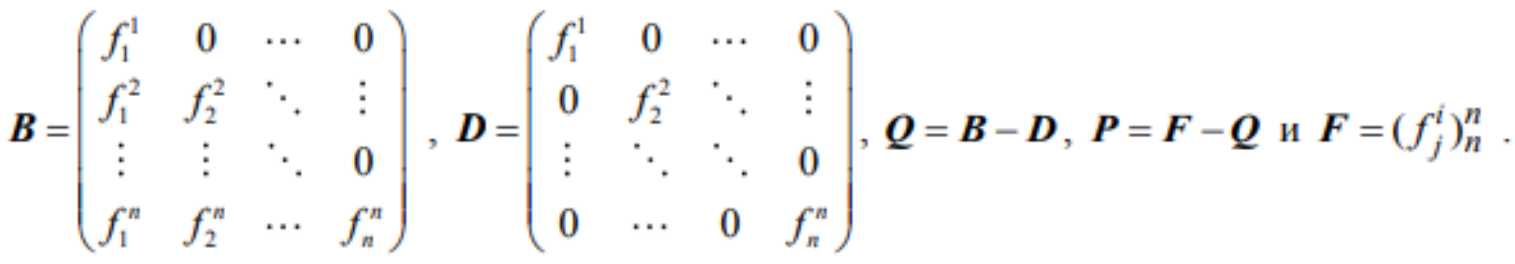
\includegraphics[width=0.9\linewidth]{../img/eq1.png}}
\end{figure}

Тогда:
\begin{equation*}
\prescript{>}{}{y_{(k)}} = (E-Q)^{-1} \cdot P \cdot \prescript{>}{}{y_{(k-1)}} + (E-Q)^{-1} \cdot \prescript{>}{}{g}, \quad k \in \mathbb{N}
\end{equation*}

$||F|| = 0.50 < 1 \Rightarrow $ метод Зейделя сходится к решению СЛАУ.

$$ B =
\begin{pmatrix}
0        & 0        & 0        & 0 \\
-0,08333 & 0        & 0        & 0 \\
-0,16667 & -0,25    & 0        & 0 \\
-0,25    & -0,16667 & -0,08333 & 0
\end{pmatrix}
$$

$$ D =
\begin{pmatrix}
0 & 0 & 0 & 0 \\
0 & 0 & 0 & 0 \\
0 & 0 & 0 & 0 \\
0 & 0 & 0 & 0
\end{pmatrix}
$$

$$ Q =
\begin{pmatrix}
0        & 0        & 0        & 0 \\
-0,08333 & 0        & 0        & 0 \\
-0,16667 & -0,25    & 0        & 0 \\
-0,25    & -0,16667 & -0,08333 & 0
\end{pmatrix}
$$

$$ P =
\begin{pmatrix}
0 & -0,08333 & -0,16667 & -0,25    \\
0 & 0        & -0,25    & 0,166667 \\
0 & 0        & 0        & -0,08333 \\
0 & 0        & 0        & 0   
\end{pmatrix}
$$

Начальный вектор итераций:
$$
\prescript{>}{}{y_0} = 
\begin{pmatrix}
0 \\
0 \\
0 \\
0
\end{pmatrix}
$$


Получающаяся последовательность приближенных решений СЛАУ:

$$
\prescript{>}{}{y_1} = 
\begin{pmatrix}
1,5      \\
1,041667 \\
0,989583 \\
0,868924
\end{pmatrix}
\quad
\Delta\prescript{>}{}{y_1} = 0,50
$$

$$
\prescript{>}{}{y_2} = 
\begin{pmatrix}
1,031033 \\
0,978172 \\
1,011208 \\
0,994946
\end{pmatrix}
\quad
\Delta\prescript{>}{}{y_2} = 0,0310
$$

$$
\prescript{>}{}{y_3} = 
\begin{pmatrix}
1,001214581\\
0,996254446\\
1,001155145\\
1,000224352
\end{pmatrix}
\quad
\Delta\prescript{>}{}{y_3} = 0,0037
$$

Таким образом, для достижения абсолютной погрешности, не превосходящей 0.01 методом Зейделя, нам потребовалось 3 итерации. То есть метод Зейделя дал нам более быструю сходимость.


\subsection*{Задание 2}
\textbf{Задание.}\\
C погрешностью, не превосходящей величину $\varepsilon = 0.0001$ , найти все корни уравнения:
\begin{equation*}
	\resizebox{\textwidth}{!}
	{
		$\left[N+5.2+(-1)^{N} \alpha\right] \cdot x^{3}-\left[2 N^{2}+10.4 N+(-1)^{N+1} \alpha\right] \cdot x^{2}-N^{2}(N+5.2)(x-2 N)+(-1)^{N} \alpha=0$
	}
\end{equation*}

Нарисовать график функции, стоящей в левой части уравнения. Используя этот график отделить корни уравнения. Для определения левого корня использовать метод касательных, правого – метод секущих. Для определения срединного корня использовать метод деления отрезка пополам.\\
\textbf{Исходные данные.}\\
$N = 6, n = 53, \alpha = 0.005(n-50) = 0.015$\\
\textbf{Решение.}\\

Исходное уравнение:
\begin{equation*}
	11.215 x^3 - 134.385 x^2 - 403.2 x + 4838.42
\end{equation*}

\begin{figure}[h]
	\centering{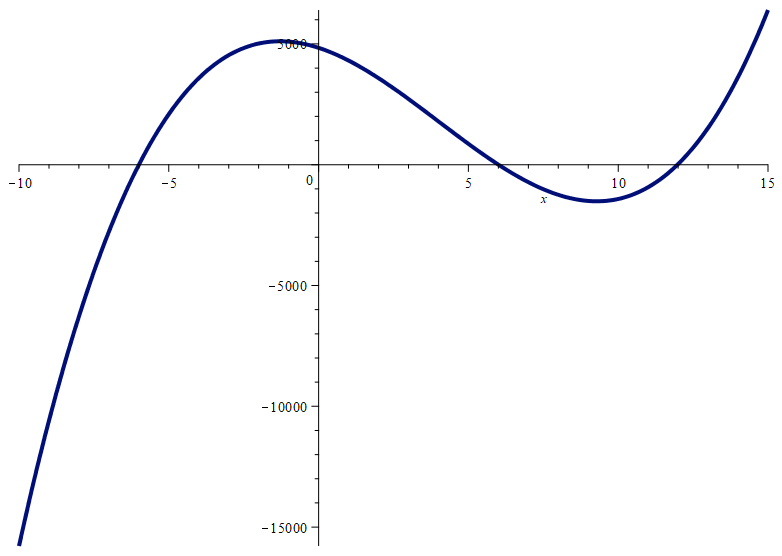
\includegraphics[width=1\linewidth]{../img/plot.png}}
	\caption{График левой части уравнения}
\end{figure}

Корни уравнения найдём с помощью сервиса WolframAlpha:
\begin{equation*}
	x_1 = -5.99889 \quad x_2 = 6.00472 \quad x_3 = 11.97680
\end{equation*}

Рабочая формула метода касательных (для определения левого корня уравнения):
\begin{equation*}
	x_{k}=x_{k-1}-\left(f^{\prime}\left(x_{k-1}\right)\right)^{-1} \cdot f\left(x_{k-1}\right)
\end{equation*}

Пусть начальное приближение $x_0 = -7$

Получающаяся последовательность приближенных корней уравнения:

\begin{equation*}
	x_1 = -6,113854602 \quad \Delta x_1 = 0,114964602
\end{equation*}
\begin{equation*}
	x_2 = -6,000683418 \quad \Delta x_2 = 0,001793418
\end{equation*}
\begin{equation*}
	x_3 = -5,998891065 \quad \Delta x_3 = 1,06466E-06
\end{equation*}

На третьей итерации достигли значения, абсолютная погрешность которого не превышает 0.0001

Для определения правого корня используем метод секущих.
Если $ f(a)\cdot f(b) < 0$ и $f(b) \cdot f'' > 0$ на $[a,b]$, то целесообразно использовать метод, не выпускающий корень $x_* \in [a,b]$ из найденной «вилки» и использующий рабочую формулу:
\begin{equation*}
	x_{k}=x_{k-1}-\frac{\left(b-x_{k-1}\right) f\left(x_{k-1}\right)}{f(b)-f\left(x_{k-1}\right)}(k \in N)
\end{equation*}
Пусть начальное приближение $x_0 = 12$ при $b = 13$

Получающаяся последовательность приближенных корней уравнения:
\begin{equation*}
	x_1 = 11,98123259 \quad \Delta x_1 = 0,00443259
\end{equation*}
\begin{equation*}
	x_2 = 11,97763924 \quad \Delta x_2 = 0,000839244
\end{equation*}
\begin{equation*}
	x_3 = 11,97694896 \quad \Delta x_3 = 0,00014896
\end{equation*}
На третьей итерации достигли значения, абсолютная погрешность которого не превышает 0.0001

Срединный корень определим методом деления отрезка пополам.

Пусть начальное приближение $a_0 = 5, b_0 = 7$
Получающаяся последовательность приближенных корней уравнения:
\begin{align*}
	a_{1} =  10.000000 \quad b_{1 }=  11.000000 \quad x_{1} =  10.000000 \quad \varepsilon_{1}=  0.005443 \\
	a_{2} =  10.000000 \quad b_{2 }=  10.500000 \quad x_{2} =  10.500000 \quad \varepsilon_{2}=  0.494557 \\
	a_{3} =  10.000000 \quad b_{3 }=  10.250000 \quad x_{3} =  10.250000 \quad \varepsilon_{3}=  0.244557 \\
	a_{4} =  10.000000 \quad b_{4 }=  10.125000 \quad x_{4} =  10.125000 \quad \varepsilon_{4}=  0.119557 \\
	a_{5} =  10.000000 \quad b_{5 }=  10.062500 \quad x_{5} =  10.062500 \quad \varepsilon_{5}=  0.057057 \\
	a_{6} =  10.000000 \quad b_{6 }=  10.031250 \quad x_{6} =  10.031250 \quad \varepsilon_{6}=  0.025807 \\
	a_{7} =  10.000000 \quad b_{7 }=  10.015625 \quad x_{7} =  10.015625 \quad \varepsilon_{7}=  0.010182 \\
	a_{8} =  10.000000 \quad b_{8 }=  10.007812 \quad x_{8} =  10.007812 \quad \varepsilon_{8}=  0.002370 \\
	a_{9} =  10.003906 \quad b_{9 }=  10.007812 \quad x_{9} =  10.003906 \quad \varepsilon_{9}=  0.001536 \\
	a_{10} =  10.003906 \quad b_{10 }=  10.005859 \quad x_{10} =  10.005859 \quad \varepsilon_{10}=  0.000417 \\
	a_{11} =  10.004883 \quad b_{11 }=  10.005859 \quad x_{11} =  10.004883 \quad \varepsilon_{11}=  0.000560 \\
	a_{12} =  10.005371 \quad b_{12 }=  10.005859 \quad x_{12} =  10.005371 \quad \varepsilon_{12}=  0.000072 \\
\end{align*}

На четырнадцатой итерации достигли значения, абсолютная погрешность которого не превышает 0.0001

В итоге можем сделать вывод, что метод касательных и метод секущих дают быстрое приближение результата к истинному значению, метод деления отрезка пополам -- сильно уступает по скорости сходимости.


\subsection*{Приложение}
Код метода деления отрезка пополам в Python3.6
\begin{minted}{Python}
import math

func_glob =  lambda x: 15.215*x**3-303.985*x**2-1520*x+30400.015
def half_divide_method(a, b, f, theor, e):
	x = (a + b) / 2
	ind = 1
	while math.fabs(theor - x) >= e:
		x = (a + b) / 2
		a, b = (a, x) if f(a) * f(x) < 0 else (x, b)
		print('\n',ind,"a_" + str(ind) + " = ",a,
		 "\\quad b_" + str(ind), " = " , b, 
		 "\\quad x_" + str(ind) + " = ",x, "\\quad
		  \\varepsilon = ", math.fabs(theor - x), "\\\\", '\n')
	ind += 1
	return (a + b) / 2

a = 9
b = 11
theor = 10.00544265
e = 0.001
half_divide_method(a, b, func_glob, theor, e)
\end{minted}









\end{document}